
\section{Máquinas virtuais versus \conts}

A virtualização, nomeadamente sob a forma de Máquinas Virtuais é uma tecnologia que se encontra presente 
em múltiplos sistemas em produção. Esta tem progredido maioritariamente devido á sua vasta utilização no contexto empresarial, as primeiras ocorrências desta surgiram na década de 1960 e atualmente ainda se encontram em desenvolvimento. Num entanto, recentemente surgiram novas tecnologias de virtualização com a introdução do  \lincont em 2013. Esta nova tecnologia trouxe consigo uma solução mais leve em termos de recursos exigidos, mas à custa de uma virtualização mais fraca e uma maior dependência do sistema do \textit{host}. 
A vertente de emulação de containers é referida sempre num ambiente \textit{linux} com o \textit{Docker} como solução de \conts. Esta decisão é tomada visto que as soluções para Windows e macOS passam pela implementação de um hipervisor sobre o sistema operativo correspondente que, neste caso de comparação entre as duas tecnologias, não faria sentido comparar uma implementação de containers que não corresponda a todo o potencial da solução.

Segue-se uma imagem que ilustra as diferenças dos sistemas de emulação de uma forma simples.

\discutir{ref da imagem: https://www.spantree.net/blog/2015/04/29/10-things-to-know-about-docker.html}

\begin{figure}[H]
	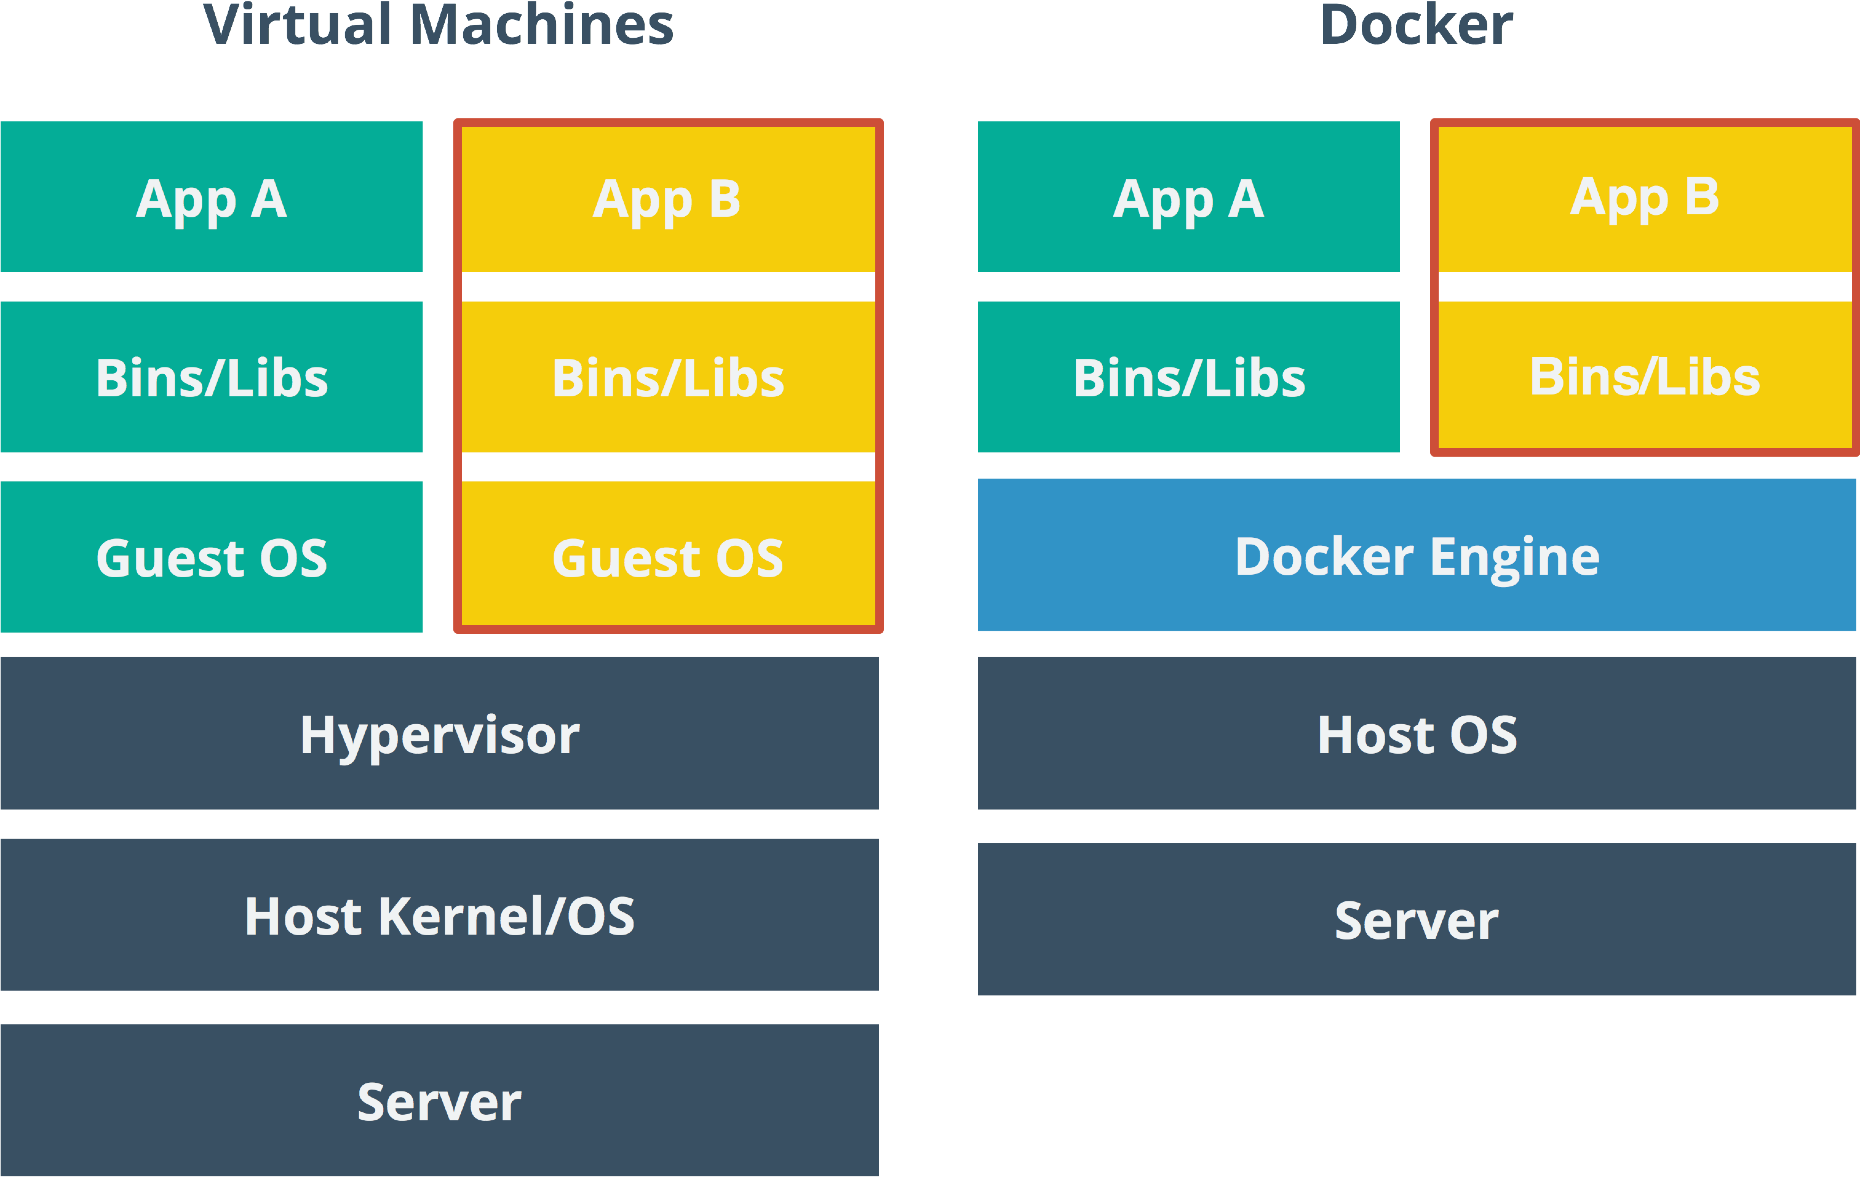
\includegraphics[width=\linewidth]{figures/docker-vs-virtual-machines.png}
	\caption{Estrutura das duas soluções de emulação}	
	\label{fig:vms-conts}
\end{figure}

\subsection{Máquinas Virtuais}

Num ambiente de virtualização por recurso a máquinas virtuais, o foco principal cai sobre o hipervisor. Este é o componente fundamental que se responsabiliza por ocultar o sistema \textit{host} e disponibilizar apenas os recursos definidos à máquina virtual, virtualizando assim um subsistema do \textit{hardware} que se apresentam como os recursos disponíveis para a mesma.

\subsection{\Conts } \label{section_conts}

A tecnologia dos \conts baseia-se numa virtualização ao nível do sistema de operação através dos \textit{control groups} e \textit{kernel namespaces} presentes no \textit{linux}, isto permite que várias instâncias de \conts possam ser executadas sobre o mesmo kernel, evitando assim a camada de virtualização do \textit{hardware} presente nas máquinas virtuais. Como referido anteriormente, a tecnologia Docker, utilizada como opção do ambiente de containers, domina atualmente o mercado no que toca a este tipo de virtualização. Num entanto, embora em constante progresso, a segurança destes ainda é um fator de preocupação.

\subsection{Conclusões}

Em suma as principais diferenças entre as duas opções de virtualização resumem-se no consumo e necessidade de recursos por instância, isolamento entre instâncias e no nível de abstração e independência do sistema \textit{host}. De notar que outras diferenças como por exemplo o tempo de arranque, espaço consumido em disco e até as ferramentas disponibilizadas pelos autores das tecnologias também contribuem para  as diferenças das tecnologias, ainda que não sejam fatores decisivos. Podemos então afirmar que o \textit{overhead} introduzido pelo hipervisor e pelo sistema operativo do \textit{guest} é determinante na performance, o qual não existe nos \conts, como já mencionadas em \ref{section_conts}. Apesar disto, a necessidade de isolamento entre processos em sistemas em produção é um fator crítico, talvez seja por isto que até á data (2018), a maioria dos sistemas em produção se encontram implementados num sistema de máquinas virtuais.

Segue-se uma tabela que de uma forma sucinta apresenta as principais diferenças.

\begin{figure}[H]
	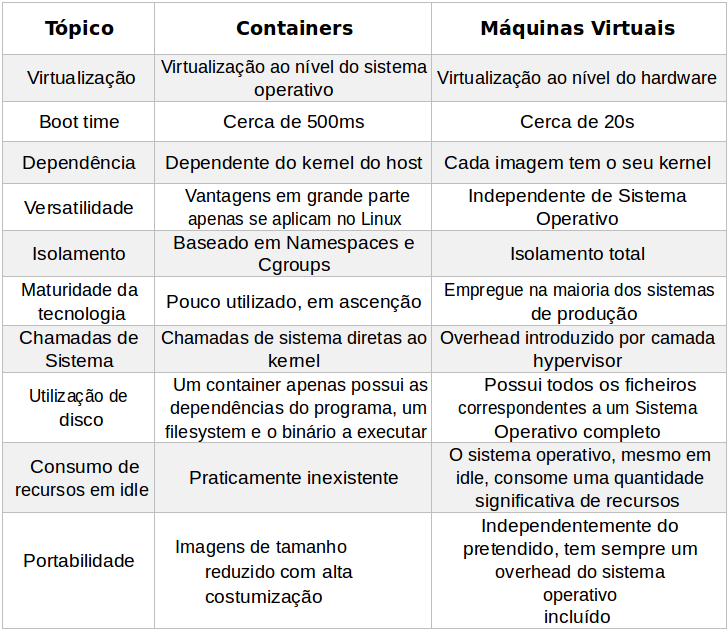
\includegraphics[width=\linewidth]{figures/tabela.png}
	\caption{Principais diferenças entre máquinas virtuais e containers}
	\label{fig:vms-conts-tabela}
\end{figure}
